
%%%%%%%%%%%%%%%%%%%%%%%%%%%%%%%%%%%%%%%%%%%%%%%%%%%%%%%%%%%%%%%%%%%%%%%%%%%%%%%%%%%%%%%
%%%%%%%%%%%%%%%%%%%%%%%%%%%%%%%%%%%%%%%%%%%%%%%%%%%%%%%%%%%%%%%%%%%%%%%%%%%%%%%%%%%%%%%
% 
% This top part of the document is called the 'preamble'.  Modify it with caution!
%
% The real document starts below where it says 'The main document starts here'.

\documentclass[12pt]{article}

\usepackage{amssymb,amsmath,amsthm}
\usepackage[top=1in, bottom=1in, left=1.25in, right=1.25in]{geometry}
\usepackage{fancyhdr}
\usepackage{enumerate}
\usepackage{listings}
\usepackage{graphicx}
\usepackage{float}

\usepackage{mwe}
\usepackage{caption}
\usepackage{subcaption}
% Comment the following line to use TeX's default font of Computer Modern.
\usepackage{times,txfonts}



\makeatletter
\renewcommand*\env@matrix[1][*\c@MaxMatrixCols c]{%
  \hskip -\arraycolsep
  \let\@ifnextchar\new@ifnextchar
  \array{#1}}
\makeatother

\newtheoremstyle{homework}% name of the style to be used
  {18pt}% measure of space to leave above the theorem. E.g.: 3pt
  {12pt}% measure of space to leave below the theorem. E.g.: 3pt
  {}% name of font to use in the body of the theorem
  {}% measure of space to indent
  {\bfseries}% name of head font
  {:}% punctuation between head and body
  {2ex}% space after theorem head; " " = normal interword space
  {}% Manually specify head
\theoremstyle{homework} 

% Set up an Exercise environment and a Solution label.
\newtheorem*{exercisecore}{Exercise \@currentlabel}
\newenvironment{exercise}[1]
{\def\@currentlabel{#1}\exercisecore}
{\endexercisecore}

\newcommand{\localhead}[1]{\par\smallskip\noindent\textbf{#1}\nobreak\\}%
\newcommand\solution{\localhead{Solution:}}

%%%%%%%%%%%%%%%%%%%%%%%%%%%%%%%%%%%%%%%%%%%%%%%%%%%%%%%%%%%%%%%%%%%%%%%%
%
% Stuff for getting the name/document date/title across the header
\makeatletter
\RequirePackage{fancyhdr}
\pagestyle{fancy}
\fancyfoot[C]{\ifnum \value{page} > 1\relax\thepage\fi}
\fancyhead[L]{\ifx\@doclabel\@empty\else\@doclabel\fi}
\fancyhead[C]{\ifx\@docdate\@empty\else\@docdate\fi}
\fancyhead[R]{\ifx\@docauthor\@empty\else\@docauthor\fi}
\headheight 15pt

\def\doclabel#1{\gdef\@doclabel{#1}}
\doclabel{Use {\tt\textbackslash doclabel\{MY LABEL\}}.}
\def\docdate#1{\gdef\@docdate{#1}}
\docdate{Use {\tt\textbackslash docdate\{MY DATE\}}.}
\def\docauthor#1{\gdef\@docauthor{#1}}
\docauthor{Use {\tt\textbackslash docauthor\{MY NAME\}}.}
\makeatother

% Shortcuts for blackboard bold number sets (reals, integers, etc.)
\newcommand{\Reals}{\ensuremath{\mathbb R}}
\newcommand{\Nats}{\ensuremath{\mathbb N}}
\newcommand{\Ints}{\ensuremath{\mathbb Z}}
\newcommand{\Rats}{\ensuremath{\mathbb Q}}
\newcommand{\Cplx}{\ensuremath{\mathbb C}}
%% Some equivalents that some people may prefer.
\let\RR\Reals
\let\NN\Nats
\let\II\Ints
\let\CC\Cplx

%%%%%%%%%%%%%%%%%%%%%%%%%%%%%%%%%%%%%%%%%%%%%%%%%%%%%%%%%%%%%%%%%%%%%%%%%%%%%%%%%%%%%%%
%%%%%%%%%%%%%%%%%%%%%%%%%%%%%%%%%%%%%%%%%%%%%%%%%%%%%%%%%%%%%%%%%%%%%%%%%%%%%%%%%%%%%%%
% 
% The main document start here.

% The following commands set up the material that appears in the header.
\doclabel{STAT 401: Homework 7}
\docauthor{Stefano Fochesatto}
\docdate{\today}


%\begin{figure}[H]
%  \begin{center}
%  \caption{}
%  \includegraphics[\textwidth]{}
%  \end{center}
%\end{figure}

% \textbf{Code:}
% \begin{center}
% \lstinputlisting{}
% \end{center} 



\begin{document}

\begin{exercise}{1} As an extreme example of what can happen when an important predictor is excluded from a model, 
  consider the data produced by the following code:\\
 \textbf{Code:}
 \begin{center}
 \lstinputlisting[basicstyle=\small]{r1.txt}
 \end{center} 
 Fit the linear models with $x_1$ and $x_2$ first and then with $x_1$ only. Comment on what happens by filling 
 each black with one of the choices that follow it in the following paragraph. \\
\solution Fitting the MLR with $x_1$ and $x_2$ the fitting an SLR using only $x_1$. \\
\textbf{Code:}
\begin{center}
\lstinputlisting[basicstyle=\small]{r2.txt}
\end{center} 

\begin{figure}[H]
  \begin{center}
  \caption{ScatterPlots for MLR}
  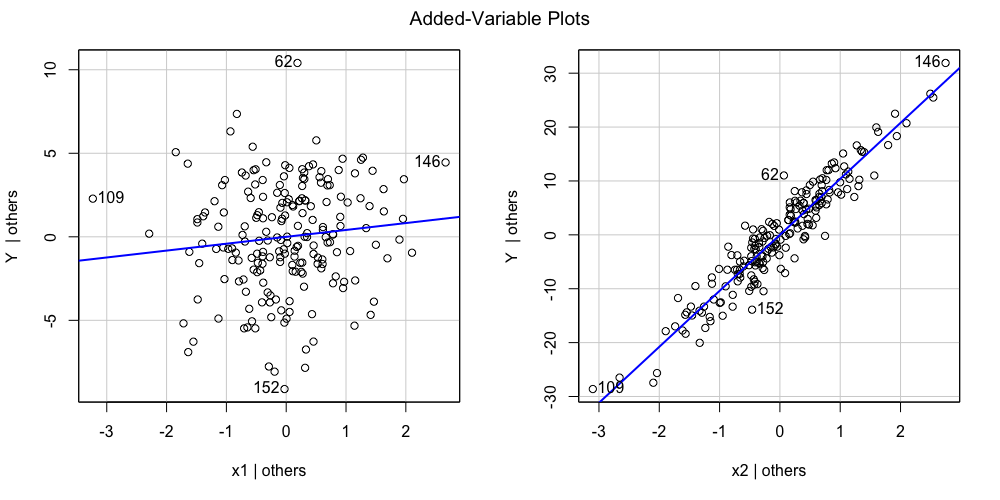
\includegraphics[width = \textwidth]{Rplot01.png}
  \end{center}
\end{figure}
\begin{figure}[H]
  \begin{center}
  \caption{ScatterPlot for SLR}
  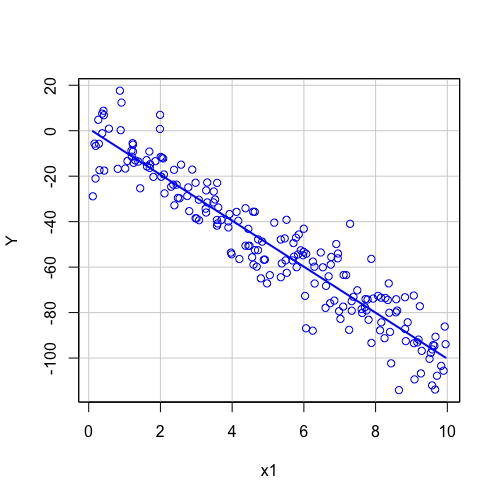
\includegraphics[width = .5\textwidth]{Rplot.png}
  \end{center}
\end{figure}



 The two models differ in that the estimated effect of $X_1$ changes from a slight \textbf{Positive}(positive/negative) 
 slope in the full model to a \textbf{steep}(steep/gradual) negative slope in the reduced model. It is clear from 
 the way the data are generated that as $X_1$ increases, the mean of \textbf{Y}$(Y/X_1/X_2)$ increases and the 
 mean of $X_2$ decreases. Hence, when $X_2$ is left out of the model, an increase in $X_1$ corresponds to an 
 uncontrolled \textbf{decrease} (increase/decrease) in $X_2$ so that $Y$ responds to both movements. Since the association
between $Y$ and$X_2$ is very strong, the effect of the increase in $X_1$ is swamped by the effect of the decrease
in $X_2$ and the mean of \textbf{Y}$(Y/X_1/X_2)$ decreases.This effect is (incorrectly) imputed, by the reduced model, 
to \textbf{X1}$(Y/X1/X2)$ since it is the only term in the model.\\
\end{exercise}
\newpage

\begin{exercise}{4.2} The data in this example consists of a sample of branches of a large Australian bank. 
  Each branch makes transactions of two types, and for each of the branches we have recorded the number $t1$ 
  of type 1 transactions and the number $t2$ of type 2 transactions. The response is time, the total minutes 
  of labor used by the branch.\\
  Define $a = (t1 + t2)/2$ to be the average transaction time, and $d = t1-t2$, and fit the following four mean functions, 
  \begin{equation*}
    M1:E(time|t1,t2) = \beta_{01} + \beta_{11}t1 + \beta_{21}t2
  \end{equation*} 
  \begin{equation*}
    M2:E(time|t1,t2) = \beta_{02} + \beta_{32}a + \beta_{42}d
  \end{equation*} 
  \begin{equation*}
    M3:E(time|t1,t2) = \beta_{03} + \beta_{23}t2 + \beta_{43}d
  \end{equation*} 
  \begin{equation*}
    M4:E(time|t1,t2) = \beta_{04} + \beta_{14}t1 + \beta_{24}t2 + \beta_{24}a + \beta_{44}d
  \end{equation*} 
  \textbf{Code:}
  \begin{center}
  \lstinputlisting[basicstyle=\footnotesize]{r3.txt}
  \end{center} 
  \newpage

  \begin{enumerate}

    \item[4.2.1] In the fit of $M4$, some of the coefficients estimates are labeled as 'aliased' or else
    they are simply omitted. Explain what this means and why this happens.\\ 
    \solution This happens because our model is overparamaterized. We have two parameters, $a, d$ which have been 
    included in the model that were computed as a linear combination of $t1, t2$. Analytically, this happens because in 
    the OLS estimator equation $(X^TX)$ is ill-conditioned(no inverse), because our design matrix does not have a full rank column space.
    \newpage
    \item[4.2.2] What aspects of the fitted regressions are the same? What aspects are different?\\
    \solution For all regressions, all coefficients have very high significance. The intercept coefficient is the same among all models. The $R-squared$
    values among all models are all the same, as well as the omnibus $F$-test. In terms of differences it seems like only the coefficients are different between 
    the models.
    \newpage
    \item[4.2.3] Why is the estimate for $t2$ different in M1 and M3?\\
    \solution Consider the M1 model, 
    \begin{equation*}
    M1:E(time|t1,t2) = \beta_{01} + \beta_{11}t1 + \beta_{21}t2.
    \end{equation*}
    Now consider the M3 model, 
    \begin{equation*}
      M3:E(time|t1,t2) = \beta_{03} + \beta_{23}t2 + \beta_{43}d
    \end{equation*} 
    Recall the definition $d=t1-t2$, by substitution into M3 we get, 
    \begin{align*}
      M3:E(time|t1,t2) &= \beta_{03} + \beta_{23}t2 + \beta_{43}(t1 - t2)\\
      &= \beta_{03} + \beta_{23}t2 + \beta_{43}t1 - \beta_{43}t2\\
      &= \beta_{03} + (\beta_{23}-\beta_{43})t2 + \beta_{43}t1
    \end{align*} 
    Looking at the models we can see that $\beta_{23}-\beta_{43} = \beta_{21}$ and $\beta_{11} = \beta_{43}$. So the difference between the coefficients
    is meant to take into account the interaction represented in $d$.
     
  \end{enumerate}
\end{exercise}
 \newpage

 \begin{exercise}{3.} The $cruise.csv$ file on canvas contians data on 158 cruise ships in operation worldwide as of
  2013. We will use $Capacity$ as the response and $Length$ and $Crew$ as predictors. Download the data and do the following.\\
  \begin{enumerate}
    \item[a.] Fit the model with both predictor and their interaction. Perform a test on the significant of the 
    interactions coefficients, including a test statistic and p-value,\\
    \solution Fitting the model and producing the t-test on the interaction coefficient we get a high significant coefficient. We get a 
    similar p-value when we use the partial F-test comparing the model with the interaction and the model without. \\
    \textbf{Code:}
    \begin{center}
    \lstinputlisting[basicstyle=\footnotesize]{r4.txt}
    \end{center}
    \newpage

    \item[b.] Interpret the interaction's estimated effect by finishing the following sentence. \\
    \solution For every additional hundred feet of length of a ship, the mean passenger capacity increases by $\textbf{1.37969 + 0.15810(4)}$
    when there are 4 hundred crew, by $\textbf{1.37969 + 0.15810(8)}$ when there are 8 hundred cre, and by $\textbf{1.37969 + 0.15810(12)}$ when there are 12 hundred crew. 
    \newpage

    \item[c.] Perhaps the interaciton is significant because increasing the lengths of ships that serve high-end customers
    does not increase capacity much, while increasing lengths of ships that serve low-end customers makes a bigger difference for capacity. But 
    the inter-relationships between all the variables makes it hard to know. To reduce these interrelationships, calculate a new 
    variable CPP by dividing Crew by Capacity. CPP is now a good proxy variable for the 'fancy-ness' of the ship. Fit the model that contains 
    Capacity, Length, and CPP, and the interaction between Length and CPP. Repeat Part b by completing the following sentence\\
    \solution For every additional hundred feet of length of a ship, the mean passenger capacity increases by $\textbf{8.4645  -9.0211(.3)}$
    when there are .3 crew per passenger, by $\textbf{8.4645  -9.0211(.5)}$ when there are .5 crew per passenger, and by $\textbf{8.4645  -9.0211(.7)}$ when there are .7 crew per passenger.\\
    Fitting the model in r we get, \\
    \textbf{Code:}
    \begin{center}
    \lstinputlisting[basicstyle=\footnotesize]{r5.txt}
    \end{center}
    Does this model support our theory? Yes, as the 'Fancy-ness' of the ship increase we see the mean passenger capacity decrease, because the interaction 
    coefficient is negative. This model confirms our theory that ships with 'High-end' customers(and therefore more crew) have smaller passenger capacity. 
    \newpage
    
    \item[d.] In a scatter plot matrix of $Capacity$, $Length$, and $CPP$, there appears to be trends between $Length$ and 
    $Capacity$ and also between $Length$ and $CPP$. Find the variance inflation factors for these in the interaction model you just fit.
    What do they tell you?\\
    \solution First let's consider the scatter plot matrix for $Capacity$, $Length$, and $CPP$.
    \begin{figure}[H]
      \begin{center}
      \caption{Scatterplot Matrix for $Capacity$, $Length$, and $CPP$ }
      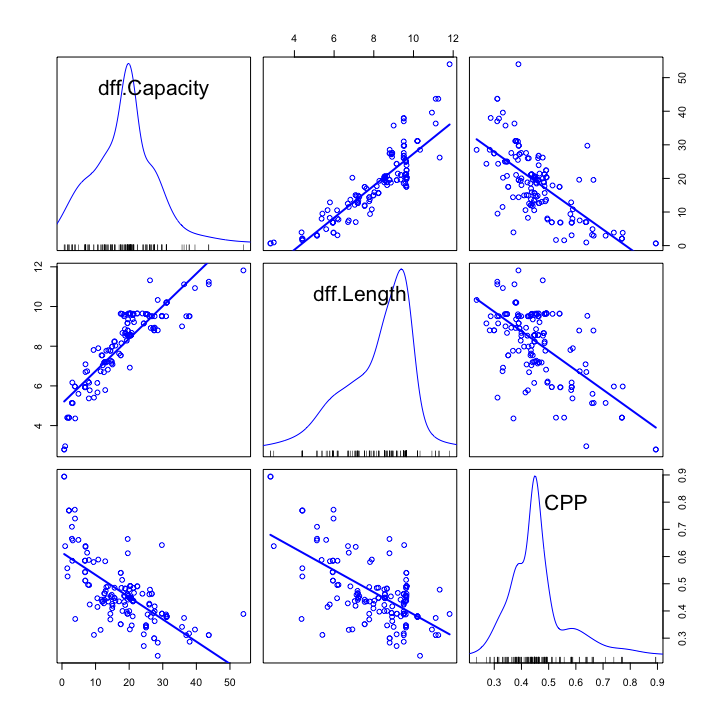
\includegraphics[width = .9\textwidth]{Rplot02.png}
      \end{center}
    \end{figure}
    Computing the variance inflation factors for the interaction model in r,\\ 
    \textbf{Code:}
    \begin{center}
    \lstinputlisting[basicstyle=\footnotesize]{r6.txt}
    \end{center}
    We use the variance inflation factors to asses collinearity between variables in the model. With values higher than 5, and around 10 our model has 
    high collinearity between all variables in the model. 



  \end{enumerate}
   
 \end{exercise}


\end{document}





















